\documentclass{report}
\usepackage{graphicx}
\usepackage{wrapfig}
\usepackage{hyperref}

\usepackage{sidecap}
\usepackage{verbatimbox}
\setlength{\topmargin}{-.5in}
\setlength{\textheight}{9in}
\setlength{\oddsidemargin}{.125in}
\setlength{\textwidth}{6.25in}


\title{CS 251 Project Report by Group 17 Sumatokoda}


\begin{document}

{\bf \centerline {Report of Box2D project (RUBE GOLDBERG MACHINE-CS251)}}  
{\centerline {Guide:{\bf {Prof.Sharat Chandran}}, Dept.of CSE, IIT Bombay}} 
{\bf \centerline{Group 17-Sumatokoda}} 
{\centerline {K.SINDHURA-140050051}} 
{\centerline {SOWMYA MUTYALA-140050072}} 
{\centerline {SHACHI DESHPANDE-140110047}}


\section{What is our project?}
We made a Rube GoldBerg Machine using Box2D,a 2D rigid body simulation library.We named it {\bf {The SWAG Machine}}.We named it so because ultimatly after simulation the word SWAG appers on the screen.In addition to this it provides food and drinks for the human sitting below.  \\ \\
\section{Our original project idea!}
In our project we were going to use dominos,pulley system,balloons,pendulums,planks,balls,containers,funnel,conveyor belts,motor system,human design,pascals system(which follows pascals law)..etc as major components in our project.Ultimately our major goal is to provide food and drinks for the human and the word SWAG to appear finally in the simulation.\\
 Initially there exists a pendulum oscillatinng in the left-top which triggers the movement of dominos on the left and a ball on the right.\\
 On the left side the movement of a domino triggers the movement of all other dominos on the first plank and the last domino on the plank is hinged to it.Similarly this last domino triggers the other dominos on the second plank and ultimately leading to the formation of S.And the movement of the block on the third plank is triggered by the last domino on the third plank.This falls on the conveyor belt below and sensors are used to detect the collision between the block and conveyor belt and give it a force towards right.This block hits the ball which in turn hits the domino on its right and the movement of dominos ultimately leading to the formation of half part of A.\\ \\
 On the right side when the bob of pendulum hits the ball the ball bounces two times on the two horizontal planks in W and after final bounce it goes through passage in D and hits the block.This block falls on the rotating motor and ultimately the block falls in the conveyor belt whose movement leads to the formation of another half part of A as described above.\\
 This completes the SWAG formation.\\ 
 Coming to the food and drinks to be provided to the human,this implementation starts below the SWAG.The balls in the left most container below SWAG leak through the gap and through the passage they go into the right container of the pulley system.While this right container is moving up it hits the plank on its right and with the movement of hot air balloons this moves and triggers the movement of plank on which drinks are placed.This completes providing drinks to the human.\\ 
 On the right side below the SWAG a heavy ball near G is triggered by the rotating motor which passes through the funnel and this heavy ball pushes the food in the right container and using the conclusions of Pascal's law the food comes out from the passage in the left container and ultimately goes into the bowl near human.This completes the total implementation.\\ 
 \newpage
\section{Original Project Design}

\begin{figure}[h]
	\begin{center}
	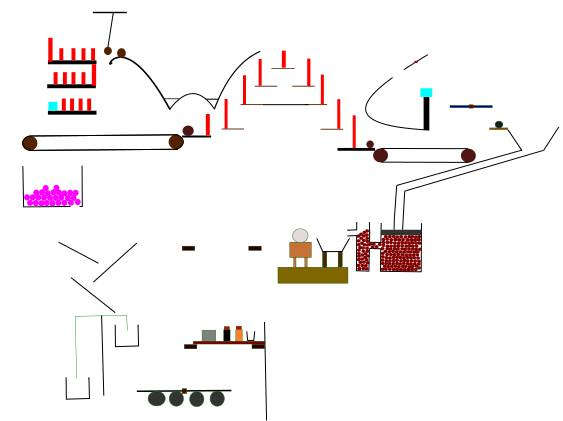
\includegraphics{./doc/pd.jpg}
	\end{center}
\end{figure}



\newpage
\section{Final project implementation}

\section{Major Components in our project}

\subsection{Simple Pendulum}
\begin{wrapfigure}{r}{0.4\textwidth}
	\caption{A picture of simple pendulum}
	\begin{center}
	 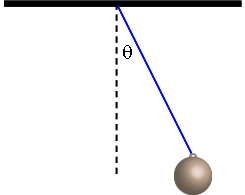
\includegraphics[width=0.2\textwidth]{./doc/pendulum.png}%
	 \end{center}
	
\end{wrapfigure}

\begin{frame}
\centering


\begin{flushleft}

\end{flushleft}
Our project starts with an oscillating simple\\ pendulum giving impulse to a domino placed\\ on one side of it and a ball placed on other side of it.\\ \\ \\ \\ \\
\end{frame}

%%%%%%%%%%%%%%%%%%%%%%%%%%%%%%%%%%%%%%%%%%%%%%%%%%%%%%%%%%%%%%%
\subsection{Conveyor belt}
\begin{wrapfigure}{r}{0.4\textwidth}
	\caption{A picture of conveyor belt}
	\centering
	 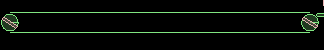
\includegraphics[width=0.2\textwidth]{./doc/conveyor.png}%
\end{wrapfigure}
\begin{frame}
\centering
\\
Conveyor in our project is used to carry\\ a block which triggers a mechanism . \\
Here whenever an object falls on\\ the conveyor belt we used sensors to \\detect the object and give it a force to the \\left or right accordingly.\\We introduced there two rotating motors to\\ give the effect of conveyor belt. 
\end{frame}


%%%%%%%%%%%%%%%%%%%%%%%%%%%%%%%%%%%%%%%%%%%%%%%%%%%%%%%%%%%%%%%
\subsection{Pressure transfering system}
\begin{wrapfigure}{r}{0.4\textwidth}
	\caption{A picture of pressure tranfering system}
	\centering
	 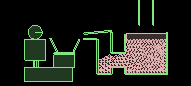
\includegraphics[width=0.2\textwidth]{./doc/pascal.png}%
\end{wrapfigure}
\begin{frame}
\centering
\\
\\
In this system when we give pressure on \\a larger surface on the plunger above popcorn (balls) \\on right using a heavy ball that comes through the channel \\above it. This pressure gets equally\\ distributed and the popcorn (balls)\\ filled inside the box are squeezed. They get pushed and emerge\\ from the left funnel and get delivered into man's bowl to the left \\of the system. This collection of static rectangular objects to the left\\ of this system represents man sitting on chair with a table holding bowl, \\ready to eat things that are delivered from the funnel.
\end{frame}
\\
\\
\\
\\
%%%%%%%%%%%%%%%%%%%%%%%%%%%%%%%%%%%%%%%%%%%%%%%%%%%%%%%%%%%%%%%
\newpage
\subsection{Balloon System}
\begin{wrapfigure}{r}{0.4\textwidth}
	\caption{A picture of balloon system}
	\centering
	 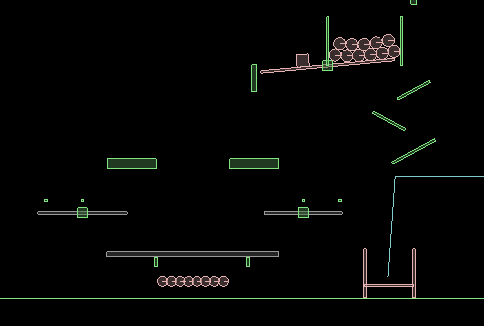
\includegraphics[width=0.2\textwidth]{./doc/balloon.png}%
\end{wrapfigure}
\begin{frame}
\centering
\\
\\
We made this balloon system simulation\\by introducing the negative gravity because of \\which they move upward to trigger \\the few dynamic bodies to get lifted. This will further \\stimulate the balls in upper container to fall \\and stimulate pulley. The upper container containing balls has an \\opening which is blocked by a motor of zero angular velocity and high torque. \\The negative gravity balls slowly accumulate on left pane of the motor and\\ push it so as to unblock the opening and allow the \\balls to fall in pan of pulley.
\end{frame}
\\
\\
%%%%%%%%%%%%%%%%%%%%%%%%%%%%%%%%%%%%%%%%%%%%%%%%%%%%%%%%%%%%%%
\subsection{Rotating Motor}
\begin{wrapfigure}{r}{0.4\textwidth}
	\caption{A picture of rotating motor}
	\centering
	 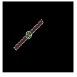
\includegraphics[width=0.2\textwidth]{./doc/motor.jpg}%
\end{wrapfigure}
\begin{frame}
\centering
\\
\\
We have introduced Revolute Joint and enabled \\the motor property.We have given that\\ motor an angular speed and required torque\\ accordingly. Such motors have been used in our project \\to provide required momentum to balls moving along in simulation.
\end{frame}
\\
\\
%%%%%%%%%%%%%%%%%%%%%%%%%%%%%%%%%%%%%%%%%%%%%%%%%%%%%%%%%%
\subsection{Letter S}
\begin{wrapfigure}{r}{0.4\textwidth}
	\caption{A picture of hinge system}
	\centering
	 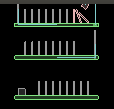
\includegraphics[width=0.2\textwidth]{./doc/S.png}%
\end{wrapfigure}
\begin{frame}
\centering
\\
\\
Basically S letter is made of 3 horizontal planks one below\\ the other, upon which train of dominos is kept.
The topmost \\domino is stimulated by the pendulum described above. \\This leads to a chain reaction making all dominos fall.
We \\implemented Revolute Joint to give the effect of\\ hinge.It takes one anchor and two objects\\ and connects the two objects with the\\ thread through the point.We defined\\ one of the objects as a dynamic rod and other\\ as a small static object with the anchor point\\ on itself which gives the effect\\ of hinge.So, when dominos fall off on the horizontal planks in 'S', the last domino to fall on each plank is hinged in this way to the tip of horizontal plank. So it stays connected to the plank as it dangles down to the area above lower plank. This helps to stimulate dominos on the lower planks successively.
\end{frame}
\\
%%%%%%%%%%%%%%%%%%%%%%%%%%%%%%%%%%%%%%%%%%%%%%%%%%%%%%%%%%%%%
\newpage
\subsection{W letter}
\begin{wrapfigure}{r}{0.4\textwidth}
	\caption{A picture of letter W}
	\centering
	 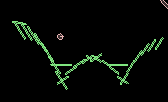
\includegraphics[width=0.2\textwidth]{./doc/W.png}%
\end{wrapfigure}
\begin{frame}
\centering
\\
\\
W letter is basically made of static rectangular blocks \\added according to parabolic trajectory defined by loop variables.\\ This is added
using 4 for-loops and the inclinations, and sizes are \\controlled by the loop variables too. Ultimately 2 horizontal planks\\ are added
at the 2 pointed parts of W letter in the bottom so that \\a ball can bounce over it and move to the next letter.
\end{frame}
\\
\\
\\

\subsection{A Letter}
\begin{wrapfigure}{r}{0.4\textwidth}
	\caption{A picture of letter A}
	\centering
	 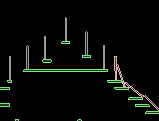
\includegraphics[width=0.2\textwidth]{./doc/A.png}%
\end{wrapfigure}
\begin{frame}
\centering
\\
\\
This is formed using a number of small static horizontal \\planks placed one near the other, and dominos stand over each\\ of these planks.
These dominos are triggered into action due to the\\ block that is delivered by conveyor. They fall one after the other \\revealing an A in the end. The leftmost domino is triggered by block \\delivered by conveyor while the rightmost domino begins to fall by \\itself in the beginning of simulation. This is done by adding small slope \\to the rightmost domino in the constructor function for the \\simulation, so that it is not in balance and falls off making all the \\leftward dominos relative to it fall one after the other.
\end{frame}
\\
\\

%%%%%%%%%%%%%%%%%%%%%%%%%%%%%%%%%%%%%%%%%%%%%%%%%%%%%%%%%%%%%

\subsection{G letter}
\begin{wrapfigure}{r}{0.4\textwidth}
	\caption{A picture of letter G}
	\centering
	 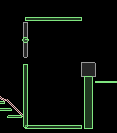
\includegraphics[width=0.2\textwidth]{./doc/G.png}%
\end{wrapfigure}
\begin{frame}
\centering
\\
\\
This letter is formed by a number of static rectangular \\bodies arranged to form this letter. The rightward stem of\\ G holds a dynamic box. There is a motor on left arm of G, which acts \\as a window for the ball which will bounce off from W and enter\\ into the letter G. This is implemented as a revolute joint again. The \\right of G is constructed so as the dynamic box kept on stem of G \\slides off and pushes the heavy ball to its right into action, and the \\heavy ball falls into the tunnel made at the right of G.
\end{frame}
\\
\\
%%%%%%%%%%%%%%%%%%%%%%%%%%%%%%%%%%%%%%%%%%%%%%%%%%%%%%%%%%%%%




\newpage

%%%%%%%%%%%%%%%%%%%%%%%%%%%%%%%%%%%%%%%%%%%%%%%%%%%%%%%%%%%%%
\subsection{Pulley system}
\begin{wrapfigure}{r}{0.4\textwidth}
	\caption{A picture of pulley system}
	\centering
	 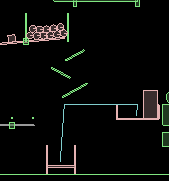
\includegraphics[width=0.2\textwidth]{./doc/pulley.png}%
\end{wrapfigure}
\begin{frame}
\centering
\\
\\
Pulley joints are used to make this system\\which takes two anchors and two objects and \\connects the two objects with the thread\\ through two points giving the effect\\ of a common balance. In our project, the right container is \\successively filled with few balls that are let into it directly. \\This creates downword force, and the pulley joint helps in\\ moving one pan up and the other down.The balls fall \\into left pan of the pulley and \\make the right pan rise up and deliver some more food to the man.
\end{frame}
\\
\\
%%%%%%%%%%%%%%%%%%%%%%%%%%%%%%%%%%%%%%%%%%%%%%%%%%%%%%%%%%%%%



\newpage
\section{Changes made in original design}
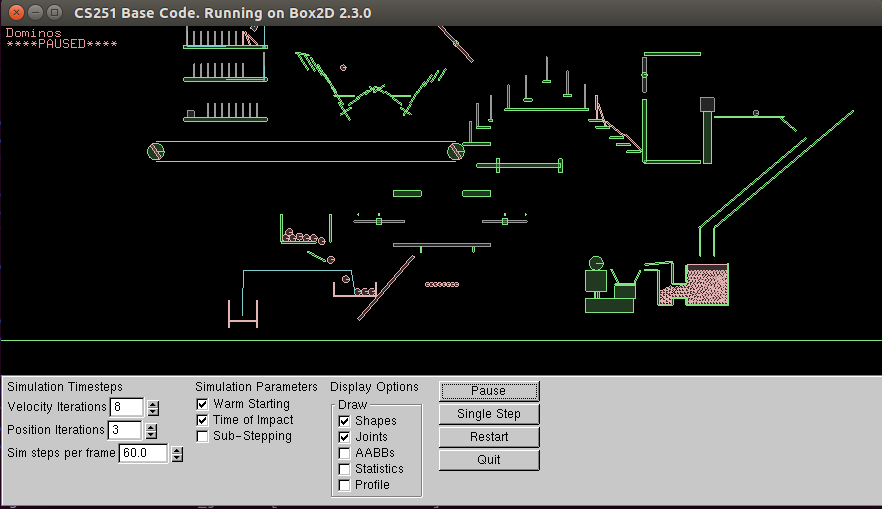
\includegraphics[scale=0.5]{./doc/final_design.png}
\newpage

\section{Changes}
Our final implementation had few changes as opposed to original project design.The changes made were as follows:\\
1. We excluded the right conveyor belt, and worked with only the left conveyor belt.\\
2. We made the 'G' letter from straight segments and not curved ones as in the original idea.\\
3. We changed the food-delivery system for the man on his left side by putting food into pan of pulley instead of making a table for that. \\
\newpage
\section{Difficulties faced and solutions devised}
We changed some parts of design due to physical constraints on motion of few objects.\\
We did not add the conveyor to right since it was very difficult to make the block on stem of G fall on it.\\
Also, due to shortage of space in the actual frame, we removed the food table on right of man, and changed that to food delivery system by a pulley joint.
Due to space constraints, we also changed the position of the assembly delivering food to man.\\
Also, we changed the curved design of G to straight segments, since implementation of curved parts was not very good to look in 
the final simulation.\\
We had a lot of problems in implementing sensors. We read a lot about sensors and collectively implemented it finally, using iforce2d tutorials for reference.
\\
While implementing Pascal's law we changed the design, and removed conveyor belt on the right.We changes the design of food-items 
serving plate in original project proposal. This helped us make changes in dimensions of the pressure-transferring system and the food-delivery from it started working well.\\
We had many problems in executing the A letter part in the simulation. We had to make hundreds of simulations to make the dominos on the 
sequential blocks fall in synchrony.In the formation of A in SWAG ,we had to change the densities of individual dominos, adjust the impulse given by block to leftmost domino by adjusting the horizontal speed of 'conveyor', and so on. Almost all these things required hundreds of simulations again and again,
changing one property at a time.\\
\newpage
\section{New Things Learnt}
We learnt following things from this lab:\\
1. Implementation of revolute joints\\
 	Revolute joints can be used in a variety of ways. They can be used to hold 2 objects, and we can define the amount of allowed rotation. We can define the points on the 2 bodies along which we want to see the rotation happening. The most wonderful thing about it is that it can be used to create motors.\\
2. Adding custom motors using revolute joints\\
 We can define specific maximum torque and angular speed for motors. These motors can be helpful to generate required impulses in the simulation.\\
3. Adding sensors:\\
	Sensors can be added by initially defining the required fixtures' isSensor value as true.Now we have to define a new sensor, overriding the BeginContact and EndContact functions in the class extending contactListener. This helps us to define the action to 
be taken when sensors come into contact. This was the key feature we used in making conveyor belt.\\
\newpage
\section{Profiling}
We used gprof tool to profile the code. We have the following observations for the same.
These are the top 3 functions who consume more time.

\begin{center}
\begin{tabular}{ ||c c c c|| } 
 \hline      
time & seconds & seconds & calls Ts/call Ts/call name  \\
40.35 & 0.23 & 0.23 & b2World::SolveTOI() \\
21.05 & 0.35 & 0.12 & b2ContactManager::AddPair() \\
14.04 & 0.43 & 0.08 & b2World::Solve() \\
 \hline
\end{tabular}
\end{center}
 
In the original base code, such top 3 functions consuming most of the time were as follows:
\begin{center}
\begin{tabular}{ ||c c c c|| } 
 \hline      
time & seconds & seconds & calls Ts/call Ts/call name  \\
10.71 & 0.03 & 0.03 & operator*() \\
7.14 &  0.05 & 0.02 & b2Dot() \\
7.14 & 0.07 & 0.02 & b2Vec2::b2Vec2() \\
 \hline
\end{tabular}
\end{center}




Since we implemented sensors in our project, more time was spent in functions related to that, like SolveTOI and b2ContactManager:: AddPair().
The efficiency of various functions did not change much after making specific changes after looking at above profiling data. 
\newpage
\section{Honor code and Contributions}
We pledge on our honour that we have not given or received any unauthorized assistance on this assignment or any previous task.\\

{\b Contributions}:\\
Each of us has contributed as much as possible. We are giving 100 percent to each of us.\\
Specifics:\\

Sindhura: \\
Completed 'S', Smiley part containing table,negative gravity balls, gprof, part of conveyor belts\\

Shachi:\\
Completed 'W', 'G' pressure-transferring system based on pascal's law, man with bowl system, Makefile, Doxygen documentation\\

Sowmya : \\
Conveyor belts, presentation, latex report, 'A' part.\\

We have helped each other in all these things mentioned above.\\
\textbf{Github link to our work}\\
https://github.com/mutant0609/Sumatokoda.git
\newpage
\section{References}

The following sites were very useful to study box2D
\cite{DUMMY:1}
\cite{DUMMY:2}\\
Following youtube links were very useful to get idea of what exciting things can be done in box2D.
\cite{DUMMY:3}
\cite{DUMMY:4}
\cite{DUMMY:5}
\cite{DUMMY:6}



\newpage

\bibliography{ProjectReport} 
\bibliographystyle{ieeetr}






\end{document}
